\documentclass[11pt]{article}

\usepackage[margin=1in]{geometry}
\usepackage{amsmath,amssymb,amsthm}
\usepackage{booktabs}
\usepackage{graphicx}
\usepackage{tikz}
\usetikzlibrary{arrows.meta, positioning}
\usepackage[colorlinks=true, linkcolor=blue!50!black, citecolor=blue!50!black, urlcolor=blue!50!black]{hyperref}
\usepackage{enumitem}

\title{\Large Analytical Insight and Numerical Precision:\\
The Interplay of Mathematical and Computational Methods\\ in Theoretical Physics}

\author{}
\date{\today}

\begin{document}

\maketitle
\vspace{-1.5em}

\begin{abstract}
\noindent Theoretical physics advances through two complementary modes of inquiry: analytical methods, which yield closed-form solutions, symmetry-based classifications, and asymptotic understanding; and numerical methods, which extract quantitative, falsifiable predictions from equations that admit no closed-form solution. This paper argues that progress in physics is best understood not as a competition between these modes but as a structured dialogue between them. We review the distinct kinds of understanding each approach supplies, and examine five case studies -- topological solitons and Derrick's theorem, lattice gauge theory and confinement, the Wilson--Fisher $\epsilon$-expansion versus Monte Carlo estimates of critical exponents, the Fermi--Pasta--Ulam--Tsingou numerical experiment and the discovery of solitons, and numerical relativity's treatment of binary black hole mergers -- in which analytic reasoning and numerical computation jointly produced results that neither could have reached alone. We then abstract general mechanisms of the interaction: how analytic structure reduces computational cost and supplies benchmarks, and how numerical experiment motivates new theorems and reveals unanticipated phenomena. We close with remarks on verification, validation, and the epistemic risks of treating either mode as self-sufficient.
\end{abstract}

\section{Introduction}

Every physical theory begins as a set of equations, and every set of equations poses the same two questions: what do these equations \emph{mean}, and what do they \emph{predict}? The first question is the province of analytical methods -- the search for symmetries, conserved quantities, exact solutions, and controlled approximations that expose the structure of a theory. The second is increasingly the province of numerical methods -- the direct, brute-force evaluation of a theory's consequences for a specific system, at specific parameter values, without an intervening closed-form expression.

For much of the history of physics these two questions had a single answer. Kepler's laws, the harmonic oscillator, the hydrogen atom, and the free electromagnetic field are all exactly solvable, so understanding and prediction coincided in a formula. This coincidence was never the rule; it was a fortunate accident of the simplest problems. Once physicists asked about three mutually gravitating bodies, a turbulent fluid, or a strongly coupled quantum field, closed-form answers vanished, and Poincar\'e's demonstration that even the three-body problem is not integrable made it clear that this was not a temporary embarrassment to be resolved by cleverer algebra, but a structural feature of nonlinear and many-body physics \cite{Poincare1890}. Understanding and prediction split apart, and they have never fully reunited.

The thesis of this paper is that this split is productive rather than merely inconvenient. Analytical methods do not become obsolete when a problem resists exact solution; they change role, supplying the scaffolding -- symmetries, bounds, limiting cases, scaling laws -- within which a numerical calculation can be designed, trusted, and interpreted. Numerical methods, in turn, do not merely fill gaps left by analysis; they routinely return results so unexpected that they force the creation of new analytical frameworks. What follows is an attempt to make this dialogue concrete: first by characterizing what each mode contributes on its own (Sections 2 and 3), then by tracing five historical episodes in which the two modes visibly depended on one another (Section 4), then by abstracting the general mechanisms at work (Section 5), and finally by considering what can go wrong when the dialogue breaks down (Section 6).

\section{Analytical Methods: The Architecture of Understanding}

\subsection{Symmetry, conservation, and exact solutions}

The deepest analytic results in physics are usually statements about what \emph{must} be true independent of the details of a calculation. Noether's theorem ties every continuous symmetry of the action to a conservation law, and this single fact organizes enormous swaths of physics -- energy, momentum, and charge conservation are not separately discovered facts about nature but consequences of time-translation, space-translation, and gauge invariance. Symmetry arguments of this kind cost nothing computationally and yet constrain the space of possible outcomes more tightly than any simulation could, because they hold exactly, for all parameter values, not merely at the points a numerical scan happens to sample.

A smaller number of problems can be solved exactly in closed form, and these exactly solvable models play a role in physics disproportionate to their number: they are the fixed points against which approximate and numerical methods are calibrated. Onsager's 1944 solution of the two-dimensional Ising model in zero field is the canonical example \cite{Onsager1944}: it demonstrated, rigorously and without approximation, that a short-range statistical model can undergo a genuine phase transition with a logarithmically divergent specific heat, settling a question that mean-field theory could not answer and giving later numerical and renormalization-group treatments of more complicated (three-dimensional, non-integrable) models a known, exact target to reproduce in the appropriate limit.

\subsection{Perturbation theory, asymptotics, and topology}

Where exact solution is unavailable, analysis still offers controlled approximation. Perturbation theory expands a solution around an exactly solvable limit in a small parameter, and even when the resulting series diverges, its low-order terms and its pattern of divergence carry information -- about the location of nearby singularities, non-perturbative scales, or the existence of Borel-resummable structure -- that no single numerical run supplies directly, because a simulation returns a number, not a functional dependence on the coupling.

A more topological form of analytic reasoning classifies field configurations by conserved integer charges -- winding numbers, homotopy classes -- that cannot change under continuous, finite-energy evolution. Such arguments can prove that a stable, particle-like solution \emph{must} exist in a given theory without ever constructing that solution, which is exactly the situation in which numerical methods become indispensable: analysis guarantees existence and stability, and computation supplies the explicit profile, mass, and interactions of the object whose existence it guarantees. Section 4.1 develops this interplay in detail.

\subsection{Where the pen and paper stop}

Analytic methods reach a wall in essentially three circumstances: strongly coupled or non-perturbative regimes, where the relevant expansion parameter is not small; genuinely nonlinear dynamics with no separation of scales, where perturbation theory around a linear or free solution fails qualitatively rather than just quantitatively; and high-dimensional or many-body systems, where the number of relevant degrees of freedom overwhelms the bookkeeping of any closed-form ansatz. The infrared behavior of quantum chromodynamics (QCD), the merger phase of a binary black hole coalescence, and the equilibrium state of a disordered many-body quantum system are all, in this sense, the same kind of problem: analytically well posed, but analytically unsolved.

\section{Numerical Methods: Quantitative Access to the Intractable}

\subsection{Discretization and direct simulation}

The generic numerical strategy is to replace a continuous field or trajectory with a finite set of numbers -- values on a lattice, coefficients in a truncated basis, particle positions in an $N$-body system -- and to evolve or extremize this finite representation with an algorithm whose error can, in principle, be driven to zero as the discretization is refined. Finite-difference and finite-element methods discretize space directly; spectral methods discretize by truncating an expansion in a basis chosen, when possible, from analytic knowledge of the problem's boundary conditions and symmetries -- a point to which Section 5.1 returns, since the choice of basis is itself an analytic input.

\subsection{Stochastic methods}

For systems with a very large number of degrees of freedom, direct enumeration is hopeless, but importance-sampling Monte Carlo methods make such systems tractable by evaluating high-dimensional sums or integrals through weighted random sampling rather than exhaustive summation. The algorithm introduced by Metropolis, Rosenbluth, Rosenbluth, Teller, and Teller in 1953 \cite{Metropolis1953} -- proposing configuration changes and accepting or rejecting them according to a detailed-balance criterion -- remains, in generalized form, the computational backbone of lattice field theory, statistical mechanics, and Bayesian inference alike.

\subsection{The limits of computation alone}

A numerical result, however precise, is a single point (or a finite grid of points) in parameter space. It does not, by itself, reveal \emph{why} a phenomenon occurs, does not automatically generalize to nearby theories, and is only as trustworthy as the analysis of its discretization error, statistical error, and finite-size effects allows -- all of which are themselves typically estimated by analytic scaling arguments. A simulation that has not been checked against a known limit, or whose convergence has not been demonstrated as resolution increases, is not yet a physical result; it is a number.

\section{Case Studies in Interdependence}

\subsection{Topological solitons: an existence proof meets a shooting method}

Consider a real scalar field $\phi$ in $D$ spatial dimensions with static energy
\begin{equation}
E[\phi] = \int d^D x \left[ \frac{1}{2}(\nabla \phi)^2 + V(\phi) \right], \qquad V \geq 0.
\label{eq:scalar-energy}
\end{equation}
Rescaling $\phi_\lambda(\mathbf{x}) \equiv \phi(\mathbf{x}/\lambda)$ sends the gradient term to $\lambda^{D-2}E_2$ and the potential term to $\lambda^D E_V$, where $E_2, E_V \geq 0$ are the values at $\lambda=1$. Stationarity of $E(\lambda)$ at $\lambda=1$ then requires
\begin{equation}
(D-2)\,E_2 + D\,E_V = 0.
\label{eq:derrick}
\end{equation}
For $D \geq 3$ every coefficient is non-negative, so Eq.~\eqref{eq:derrick} forces $E_2 = E_V = 0$: no non-trivial, finite-energy static solution can be stable. This is Derrick's theorem \cite{Derrick1964}, and it is a purely analytic result -- no simulation is needed to rule out ordinary static solitons in three spatial dimensions.

The theorem also indicates exactly where a loophole must be sought: a term that scales differently under the rescaling. Coupling the scalar to a non-Abelian gauge field introduces a field-strength term $\tfrac{1}{4}F_{ij}^aF^{a\,ij}$ whose two derivatives scale as $\lambda^{D-4}$, so that the full energy behaves as a sum of terms in $\lambda^{D-4}$, $\lambda^{D-2}$, and $\lambda^D$. In $D=3$ these are $\lambda^{-1}$, $\lambda^{1}$, and $\lambda^{3}$, and stationarity can now be satisfied with every term positive -- the Derrick obstruction is evaded. This is precisely the mechanism realized in the 't~Hooft--Polyakov monopole, a stable, finite-energy, particle-like solution of an $SU(2)$ gauge theory coupled to a triplet Higgs field \cite{Hooft1974}, and in the topologically stabilized Skyrmion of the nonlinear pion field, whose winding number is identified with baryon number \cite{Skyrme1962}.

Analysis alone establishes \emph{that} such solutions exist and are stable, via topology and scaling; it does not, in general, hand over their explicit profile. The 't~Hooft--Polyakov monopole equations are a coupled, nonlinear system of ordinary differential equations with no closed-form solution for generic couplings, and their radial profile functions are obtained numerically by shooting or relaxation methods, integrating inward and outward from the boundary conditions imposed by the topological sector until the two match. The one celebrated exception is the Bogomolny--Prasad--Sommerfield (BPS) limit, in which the potential is tuned to zero and the second-order field equations reduce to first-order Bogomolny equations that \emph{can} be solved in closed form \cite{PrasadSommerfield1975}; this exact solution is not merely a curiosity but the benchmark against which numerical solvers for the non-BPS monopole are validated, and the point from which numerical continuation in the Higgs self-coupling proceeds. The general pattern -- topology and scaling arguments guarantee existence and constrain stability, while root-finding or relaxation methods on the resulting boundary-value problem supply the quantitative profile -- recurs throughout soliton physics \cite{MantonSutcliffe2004}.

\subsection{Confinement: from a conjectured mechanism to a lattice measurement}

Asymptotic freedom -- the perturbative, analytically derived statement that the QCD coupling shrinks at short distances -- explains the ultraviolet behavior of the strong interaction with high precision. It says nothing directly about the opposite, infrared limit, where the coupling grows and perturbation theory breaks down entirely. Wilson's 1974 proposal for confinement addressed this regime analytically only in a formal strong-coupling limit: by formulating gauge theory on a Euclidean spacetime lattice, with gauge fields as link variables rather than continuum fields, he showed that a strong-coupling expansion predicts an area-law falloff for the expectation value of a rectangular Wilson loop $C$,
\begin{equation}
\langle W(C) \rangle \sim \exp\!\big(-\sigma \, A(C)\big),
\label{eq:wilson-loop}
\end{equation}
with $A(C)$ the minimal spanning area and $\sigma$ a string tension; an area law of this form implies a linearly rising potential between static color charges and hence permanent confinement \cite{Wilson1974}. But the strong-coupling expansion is not controlled all the way to the weak-coupling, continuum limit that describes real QCD, so Eq.~\eqref{eq:wilson-loop} in the physical theory is a conjecture inherited from a different corner of parameter space, not a proof.

Bridging that gap has been overwhelmingly a numerical achievement. Lattice QCD, evaluated by Monte Carlo importance sampling of exactly the kind introduced by Metropolis et al.\ \cite{Metropolis1953}, computes Wilson loops, hadron masses, and the deconfinement temperature directly from the same discretized action Wilson wrote down, extrapolated toward the continuum and infinite-volume limits. The qualitative claim -- that confinement holds in the physical, continuum theory -- was proposed analytically; its quantitative content -- the value of the string tension, the hadron spectrum, the location of the deconfinement transition -- is overwhelmingly numerical. Neither half is dispensable: without the lattice formulation and its strong-coupling analysis there would be no reason to expect an area law, and without large-scale Monte Carlo evaluation there would be no way to know whether that expectation survives all the way to the physical coupling.

\subsection{Critical phenomena: an expansion in $4-\epsilon$ dimensions meets simulation}

Renormalization-group theory explains critical phenomena as universal behavior controlled by a fixed point of the coupling flow, but the fixed point of, say, the three-dimensional Ising universality class cannot be reached by a controlled expansion in three dimensions directly. Wilson and Fisher's 1972 solution was to treat the spatial dimension $d = 4-\epsilon$ as a continuous parameter, locate a non-trivial fixed point perturbatively in $\epsilon$, and only afterward set $\epsilon \to 1$ to recover three dimensions \cite{WilsonFisher1972,WilsonKogut1974}. For the Ising universality class this expansion gives, to first order,
\begin{equation}
\nu = \frac{1}{2} + \frac{\epsilon}{12} + O(\epsilon^2), \qquad \gamma = 1 + \frac{\epsilon}{6} + O(\epsilon^2).
\label{eq:epsilon-expansion}
\end{equation}
Setting $\epsilon=1$ is, strictly, outside the radius of validity the derivation assumed, and Eq.~\eqref{eq:epsilon-expansion} is at best a first step in an asymptotic series known only to a limited number of orders.

Independent numerical work -- Monte Carlo simulation of three-dimensional Ising-class lattice models, and more recently the conformal bootstrap -- provides essentially exact values, with $\nu \approx 0.630$ and $\gamma \approx 1.237$ widely quoted in the modern literature. These numbers do two things at once: they confirm, at the level of a few percent, that even a first-order $\epsilon$-expansion captures the qualitative and semi-quantitative physics of the fixed point, and they expose exactly how far a low-order truncation of the analytic series is from the true answer, which in turn is what motivates extending the perturbative series to higher order and developing resummation techniques for it. Here the numerical result does not merely check the analytic one; it calibrates how much to trust it, and by how much to correct it.

\subsection{From a numerical surprise to an analytic theory: FPUT and the soliton}

Not every case runs from analysis to computation. In 1955, Fermi, Pasta, and Ulam used one of the first electronic computers to simulate a chain of masses coupled by weakly nonlinear springs, expecting energy initially placed in a single normal mode to spread ergodically among all modes, as equipartition would predict \cite{FermiPastaUlam1955}. It did not: the energy returned, after a finite time, almost exactly to the mode in which it started. This non-thermalization -- the Fermi--Pasta--Ulam--Tsingou (FPUT) recurrence -- was a numerical result with no analytic explanation at the time it was obtained.

The explanation came a decade later, and it came from further numerical experiment rather than from pure analysis in the first instance: Zabusky and Kruskal, studying the continuum limit of the same lattice, identified it with the Korteweg--de Vries (KdV) equation,
\begin{equation}
u_t + 6\,u\,u_x + u_{xxx} = 0,
\label{eq:kdv}
\end{equation}
and, simulating Eq.~\eqref{eq:kdv} numerically, observed localized pulses that passed through one another and re-emerged with unchanged shape and speed -- the phenomenon for which they coined the term \emph{soliton} \cite{ZabuskyKruskal1965}. This numerical discovery of exact particle-like coherence in a classical nonlinear wave equation is what motivated the subsequent analytic development of the inverse scattering transform, which proved that KdV is exactly integrable and explained both the solitons and the FPUT recurrence as consequences of an infinite tower of conserved quantities. The causal arrow here runs opposite to the confinement and soliton-stability cases above: a numerical anomaly created the demand for, and supplied the key intuition behind, an entirely new area of exact analysis.

\subsection{Numerical relativity: stitching analytic regimes together}

The gravitational two-body problem is exactly solvable only in special limits. Far from merger, the post-Newtonian expansion -- an analytic perturbation series in the orbital velocity -- describes the slow inspiral to high precision. Long after merger, black-hole perturbation theory describes the ringdown of the final black hole as a superposition of exponentially damped quasinormal modes, again an analytic, perturbative result. Between these two regimes lies the merger itself, where the two black holes' velocities and the spacetime curvature are simultaneously large, no small parameter exists, and the full, nonlinear Einstein field equations must be solved as they stand.

For decades this middle regime resisted stable numerical evolution; codes evolving the Einstein equations in the strong-field, dynamical regime routinely became numerically unstable well before two black holes could complete an orbit. Pretorius's 2005 evolution of a binary black hole spacetime through inspiral, merger, and ringdown, using a generalized-harmonic formulation of the field equations together with constraint-damping and excision techniques, was the first simulation to succeed \cite{Pretorius2005}, and it was followed within a year by independent moving-puncture methods that confirmed and extended the result. The resulting numerical waveforms were then stitched to the analytic post-Newtonian inspiral on one side and the analytic quasinormal-mode ringdown on the other, producing the hybrid waveform templates against which gravitational-wave detectors compare their data. No one of the three pieces -- perturbative inspiral, numerical merger, perturbative ringdown -- is dispensable, and the construction of a usable template bank is, by design, a joint analytic--numerical object.

\section{The Mechanics of the Interaction}

The five episodes above suggest that the relationship between analysis and computation is not a division of labor along a fixed boundary but a set of recurring mechanisms, each of which can run in either direction.

\subsection{Analysis disciplines computation}

Exploiting a symmetry reduces the effective dimensionality of a numerical problem -- a spherically symmetric monopole ansatz turns three-dimensional partial differential equations into ordinary differential equations in a single radial coordinate, which is what makes the shooting-method calculation of Section 4.1 tractable in the first place. Conserved quantities, known in closed form from Noether's theorem, provide running checks on a numerical integrator entirely independent of the equations being integrated: drift in total energy or momentum over the course of a simulation signals accumulating numerical error long before the physical output looks obviously wrong. Known asymptotic behavior guides the choice of numerical representation itself -- spectral methods converge fastest when the basis functions are matched to the analytically known smoothness and boundary behavior of the true solution, and a discretization scheme that respects an exact conservation law (a symplectic integrator, a gauge-invariant lattice action) will typically outperform one that does not, for the same computational cost.

\subsection{Computation provokes analysis}

The FPUT episode of Section 4.4 is the clearest instance of the opposite direction: an unexpected numerical result created an explanatory debt that pure analysis had no reason to anticipate, and the resulting effort to explain it produced an entirely new field, integrable systems theory, with a scope far beyond the original lattice problem. The critical-exponent numbers of Section 4.3 similarly turn a numerical result into a target: the size of the discrepancy between a low-order $\epsilon$-expansion and the numerically or bootstrap-determined value of $\nu$ is itself the quantity that motivates higher-order perturbative and resummation work. In both cases the numerical result functions less as an answer than as a question that only subsequent analysis can resolve.

\subsection{Verification, validation, and the limits of trust}

A numerical code is validated by its behavior in regimes where the analytic answer is already known -- against the Schwarzschild or linearized-wave limits before a merger simulation is trusted, against the BPS limit before a general monopole solver is trusted, against the exactly solved two-dimensional Ising model before a Monte Carlo code for a more complicated spin model is trusted. This is not a formality: it is the only available check on discretization error, coding error, and the many ways a numerical method can converge confidently to the wrong answer. Analytic results that are never confronted with data or simulation face a converse risk -- an elegant symmetry argument or a low-order perturbative calculation can quietly drift out of contact with the physical regime it was meant to describe, as very nearly happened with a literal reading of the $\epsilon$-expansion at $\epsilon=1$. Table~\ref{tab:comparison} summarizes the complementary strengths and characteristic failure modes of the two approaches.

\begin{table}[h]
\centering
\small
\begin{tabular}{@{}p{2.6cm}p{5.4cm}p{5.4cm}@{}}
\toprule
\textbf{Aspect} & \textbf{Analytical methods} & \textbf{Numerical methods} \\
\midrule
Typical output & Closed-form or perturbative functional dependence on parameters & Specific values at specific parameter points \\
Domain of validity & Exact, or controlled by a small expansion parameter & Whatever regime the simulation is run in \\
Error control & Systematic, order by order, or exact & Discretization, statistical, finite-size; requires convergence testing \\
Primary insight & Mechanism, symmetry, universality class, existence and stability & Magnitude, phase diagram, explicit profiles, precision values \\
Characteristic failure mode & Series divergence, no closed form beyond an idealized limit & Undiagnosed discretization or finite-size artifact; chaotic sensitivity \\
\bottomrule
\end{tabular}
\caption{Complementary strengths of analytical and numerical methods in theoretical physics.}
\label{tab:comparison}
\end{table}

Figure~\ref{fig:loop} depicts the resulting relationship schematically: not a one-way pipeline from theory to computation, but a closed loop in which each mode both constrains and is corrected by the other.

\begin{figure}[h]
\centering
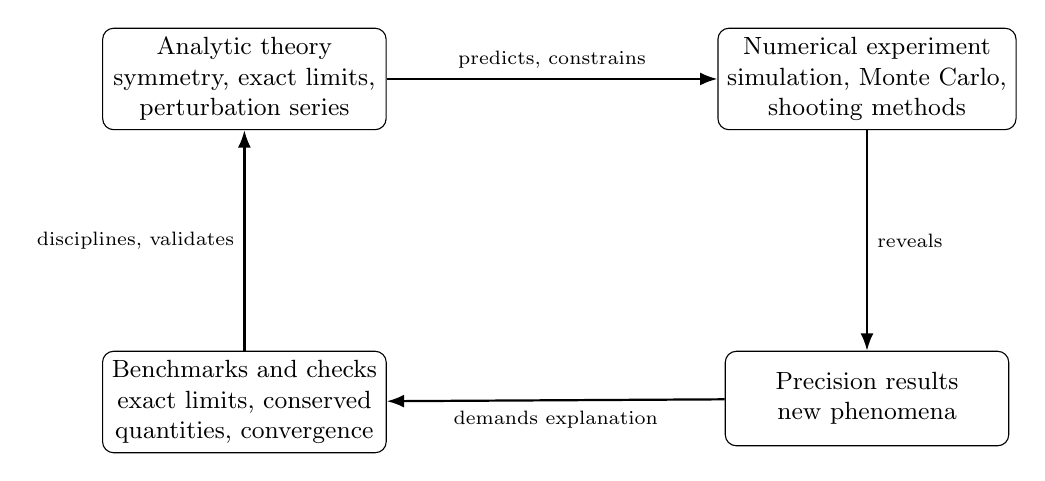
\begin{tikzpicture}[
  node distance=2.8cm and 4.2cm,
  box/.style={draw, rounded corners, align=center, minimum width=3.6cm, minimum height=1.2cm, font=\small},
  lbl/.style={font=\scriptsize, align=center},
  arr/.style={-{Latex[length=2.2mm]}, thick}
]
\node[box] (analytic) {Analytic theory\\ symmetry, exact limits,\\ perturbation series};
\node[box, right=of analytic] (numeric) {Numerical experiment\\ simulation, Monte Carlo,\\ shooting methods};
\node[box, below=of numeric] (data) {Precision results\\ new phenomena};
\node[box, below=of analytic] (validation) {Benchmarks and checks\\ exact limits, conserved\\ quantities, convergence};

\draw[arr] (analytic) -- node[lbl, above]{predicts, constrains} (numeric);
\draw[arr] (numeric) -- node[lbl, right]{reveals} (data);
\draw[arr] (data) -- node[lbl, below]{demands explanation} (validation);
\draw[arr] (validation) -- node[lbl, left]{disciplines, validates} (analytic);
\end{tikzpicture}
\caption{The interaction between analytical and numerical methods as a closed loop rather than a one-way pipeline. Each stage's output feeds the next; the benchmarking stage (Section 5.3) is where both analytic results and numerical codes are checked against known exact limits before either is trusted with a new prediction.}
\label{fig:loop}
\end{figure}

\section{Discussion: Toward a Unified Methodology}

Treating analysis and computation as rival methodologies obscures a fact that practicing physicists rely on constantly: nearly every substantial numerical result in modern physics is designed, interpreted, and trusted using analytic tools, and nearly every substantial analytic framework beyond the exactly solvable core of the subject is completed, tested, or discovered with the help of computation. General-purpose numerical software -- from Monte Carlo libraries descended from Metropolis's original algorithm to the finite-difference and spectral solvers surveyed in standard references \cite{PressNumericalRecipes2007} -- is now as much a part of a theorist's toolkit as perturbation theory or group representation theory, and increasingly the two are combined explicitly, as in numerical bootstrap methods that use exact operator-algebra constraints to bound quantities that no perturbative expansion can reach, or in machine-learning-based function approximators trained to respect known conservation laws and symmetries by construction.

The methodological lesson of the case studies in Section 4 is not that one mode is more fundamental than the other, but that the productive move is usually to ask which mode is missing at a given stage of a problem. A theory with a known symmetry but no numbers needs simulation; a numerical result with no candidate explanation needs new analysis; and a numerical code with no known limiting case against which to check its output should not yet be trusted with a genuinely new prediction.

\section{Conclusion}

Analytical and numerical methods in theoretical physics answer different questions -- why a phenomenon must occur, and what its magnitude actually is -- and neither question is dispensable. The historical record, from Derrick's scaling argument and the numerical construction of the 't~Hooft--Polyakov monopole, through Wilson's lattice formulation of confinement and its Monte Carlo verification, to the Fermi--Pasta--Ulam--Tsingou experiment that gave rise to soliton theory and the numerical relativity that finally solved the binary black hole merger, shows a discipline that has never actually separated the two modes for long. What looks, in a given decade, like a triumph of pure computation typically rests on decades of analytic groundwork that made the computation interpretable, and what looks like a purely analytic advance is, more often than the discipline's rhetoric admits, a response to something a machine found first.

\begin{thebibliography}{99}

\bibitem{Poincare1890}
H.~Poincar\'e, ``Sur le probl\`eme des trois corps et les \'equations de la dynamique,'' \emph{Acta Mathematica} \textbf{13}, 1--270 (1890).

\bibitem{Onsager1944}
L.~Onsager, ``Crystal Statistics. I. A Two-Dimensional Model with an Order-Disorder Transition,'' \emph{Phys. Rev.} \textbf{65}, 117 (1944).

\bibitem{Wilson1974}
K.~G.~Wilson, ``Confinement of Quarks,'' \emph{Phys. Rev. D} \textbf{10}, 2445 (1974).

\bibitem{WilsonFisher1972}
K.~G.~Wilson and M.~E.~Fisher, ``Critical Exponents in 3.99 Dimensions,'' \emph{Phys. Rev. Lett.} \textbf{28}, 240 (1972).

\bibitem{WilsonKogut1974}
K.~G.~Wilson and J.~B.~Kogut, ``The Renormalization Group and the $\epsilon$ Expansion,'' \emph{Phys. Rept.} \textbf{12}, 75 (1974).

\bibitem{Hooft1974}
G.~'t~Hooft, ``Magnetic Monopoles in Unified Gauge Theories,'' \emph{Nucl. Phys. B} \textbf{79}, 276 (1974).

\bibitem{Skyrme1962}
T.~H.~R.~Skyrme, ``A Unified Field Theory of Mesons and Baryons,'' \emph{Nucl. Phys.} \textbf{31}, 556 (1962).

\bibitem{Derrick1964}
G.~H.~Derrick, ``Comments on Nonlinear Wave Equations as Models for Elementary Particles,'' \emph{J. Math. Phys.} \textbf{5}, 1252 (1964).

\bibitem{PrasadSommerfield1975}
M.~K.~Prasad and C.~M.~Sommerfield, ``Exact Classical Solution for the 't~Hooft Monopole and the Julia-Zee Dyon,'' \emph{Phys. Rev. Lett.} \textbf{35}, 760 (1975).

\bibitem{MantonSutcliffe2004}
N.~S.~Manton and P.~Sutcliffe, \emph{Topological Solitons}, Cambridge Monographs on Mathematical Physics (Cambridge University Press, Cambridge, 2004).

\bibitem{Metropolis1953}
N.~Metropolis, A.~W.~Rosenbluth, M.~N.~Rosenbluth, A.~H.~Teller, and E.~Teller, ``Equation of State Calculations by Fast Computing Machines,'' \emph{J. Chem. Phys.} \textbf{21}, 1087 (1953).

\bibitem{FermiPastaUlam1955}
E.~Fermi, J.~Pasta, and S.~Ulam, ``Studies of Nonlinear Problems,'' Los Alamos Scientific Laboratory Report LA-1940 (1955).

\bibitem{ZabuskyKruskal1965}
N.~J.~Zabusky and M.~D.~Kruskal, ``Interaction of `Solitons' in a Collisionless Plasma and the Recurrence of Initial States,'' \emph{Phys. Rev. Lett.} \textbf{15}, 240 (1965).

\bibitem{Pretorius2005}
F.~Pretorius, ``Evolution of Binary Black Hole Spacetimes,'' \emph{Phys. Rev. Lett.} \textbf{95}, 121101 (2005).

\bibitem{PressNumericalRecipes2007}
W.~H.~Press, S.~A.~Teukolsky, W.~T.~Vetterling, and B.~P.~Flannery, \emph{Numerical Recipes: The Art of Scientific Computing}, 3rd ed. (Cambridge University Press, Cambridge, 2007).

\end{thebibliography}

\end{document}
